% Options for packages loaded elsewhere
\PassOptionsToPackage{unicode}{hyperref}
\PassOptionsToPackage{hyphens}{url}
%
\documentclass[
]{book}
\usepackage{lmodern}
\usepackage{amssymb,amsmath}
\usepackage{ifxetex,ifluatex}
\ifnum 0\ifxetex 1\fi\ifluatex 1\fi=0 % if pdftex
  \usepackage[T1]{fontenc}
  \usepackage[utf8]{inputenc}
  \usepackage{textcomp} % provide euro and other symbols
\else % if luatex or xetex
  \usepackage{unicode-math}
  \defaultfontfeatures{Scale=MatchLowercase}
  \defaultfontfeatures[\rmfamily]{Ligatures=TeX,Scale=1}
\fi
% Use upquote if available, for straight quotes in verbatim environments
\IfFileExists{upquote.sty}{\usepackage{upquote}}{}
\IfFileExists{microtype.sty}{% use microtype if available
  \usepackage[]{microtype}
  \UseMicrotypeSet[protrusion]{basicmath} % disable protrusion for tt fonts
}{}
\makeatletter
\@ifundefined{KOMAClassName}{% if non-KOMA class
  \IfFileExists{parskip.sty}{%
    \usepackage{parskip}
  }{% else
    \setlength{\parindent}{0pt}
    \setlength{\parskip}{6pt plus 2pt minus 1pt}}
}{% if KOMA class
  \KOMAoptions{parskip=half}}
\makeatother
\usepackage{xcolor}
\IfFileExists{xurl.sty}{\usepackage{xurl}}{} % add URL line breaks if available
\IfFileExists{bookmark.sty}{\usepackage{bookmark}}{\usepackage{hyperref}}
\hypersetup{
  pdftitle={A Primer of Ecosystem Modeling},
  pdfauthor={Hank Stevens, BIO 672},
  hidelinks,
  pdfcreator={LaTeX via pandoc}}
\urlstyle{same} % disable monospaced font for URLs
\usepackage{color}
\usepackage{fancyvrb}
\newcommand{\VerbBar}{|}
\newcommand{\VERB}{\Verb[commandchars=\\\{\}]}
\DefineVerbatimEnvironment{Highlighting}{Verbatim}{commandchars=\\\{\}}
% Add ',fontsize=\small' for more characters per line
\usepackage{framed}
\definecolor{shadecolor}{RGB}{248,248,248}
\newenvironment{Shaded}{\begin{snugshade}}{\end{snugshade}}
\newcommand{\AlertTok}[1]{\textcolor[rgb]{0.94,0.16,0.16}{#1}}
\newcommand{\AnnotationTok}[1]{\textcolor[rgb]{0.56,0.35,0.01}{\textbf{\textit{#1}}}}
\newcommand{\AttributeTok}[1]{\textcolor[rgb]{0.77,0.63,0.00}{#1}}
\newcommand{\BaseNTok}[1]{\textcolor[rgb]{0.00,0.00,0.81}{#1}}
\newcommand{\BuiltInTok}[1]{#1}
\newcommand{\CharTok}[1]{\textcolor[rgb]{0.31,0.60,0.02}{#1}}
\newcommand{\CommentTok}[1]{\textcolor[rgb]{0.56,0.35,0.01}{\textit{#1}}}
\newcommand{\CommentVarTok}[1]{\textcolor[rgb]{0.56,0.35,0.01}{\textbf{\textit{#1}}}}
\newcommand{\ConstantTok}[1]{\textcolor[rgb]{0.00,0.00,0.00}{#1}}
\newcommand{\ControlFlowTok}[1]{\textcolor[rgb]{0.13,0.29,0.53}{\textbf{#1}}}
\newcommand{\DataTypeTok}[1]{\textcolor[rgb]{0.13,0.29,0.53}{#1}}
\newcommand{\DecValTok}[1]{\textcolor[rgb]{0.00,0.00,0.81}{#1}}
\newcommand{\DocumentationTok}[1]{\textcolor[rgb]{0.56,0.35,0.01}{\textbf{\textit{#1}}}}
\newcommand{\ErrorTok}[1]{\textcolor[rgb]{0.64,0.00,0.00}{\textbf{#1}}}
\newcommand{\ExtensionTok}[1]{#1}
\newcommand{\FloatTok}[1]{\textcolor[rgb]{0.00,0.00,0.81}{#1}}
\newcommand{\FunctionTok}[1]{\textcolor[rgb]{0.00,0.00,0.00}{#1}}
\newcommand{\ImportTok}[1]{#1}
\newcommand{\InformationTok}[1]{\textcolor[rgb]{0.56,0.35,0.01}{\textbf{\textit{#1}}}}
\newcommand{\KeywordTok}[1]{\textcolor[rgb]{0.13,0.29,0.53}{\textbf{#1}}}
\newcommand{\NormalTok}[1]{#1}
\newcommand{\OperatorTok}[1]{\textcolor[rgb]{0.81,0.36,0.00}{\textbf{#1}}}
\newcommand{\OtherTok}[1]{\textcolor[rgb]{0.56,0.35,0.01}{#1}}
\newcommand{\PreprocessorTok}[1]{\textcolor[rgb]{0.56,0.35,0.01}{\textit{#1}}}
\newcommand{\RegionMarkerTok}[1]{#1}
\newcommand{\SpecialCharTok}[1]{\textcolor[rgb]{0.00,0.00,0.00}{#1}}
\newcommand{\SpecialStringTok}[1]{\textcolor[rgb]{0.31,0.60,0.02}{#1}}
\newcommand{\StringTok}[1]{\textcolor[rgb]{0.31,0.60,0.02}{#1}}
\newcommand{\VariableTok}[1]{\textcolor[rgb]{0.00,0.00,0.00}{#1}}
\newcommand{\VerbatimStringTok}[1]{\textcolor[rgb]{0.31,0.60,0.02}{#1}}
\newcommand{\WarningTok}[1]{\textcolor[rgb]{0.56,0.35,0.01}{\textbf{\textit{#1}}}}
\usepackage{longtable,booktabs}
% Correct order of tables after \paragraph or \subparagraph
\usepackage{etoolbox}
\makeatletter
\patchcmd\longtable{\par}{\if@noskipsec\mbox{}\fi\par}{}{}
\makeatother
% Allow footnotes in longtable head/foot
\IfFileExists{footnotehyper.sty}{\usepackage{footnotehyper}}{\usepackage{footnote}}
\makesavenoteenv{longtable}
\usepackage{graphicx,grffile}
\makeatletter
\def\maxwidth{\ifdim\Gin@nat@width>\linewidth\linewidth\else\Gin@nat@width\fi}
\def\maxheight{\ifdim\Gin@nat@height>\textheight\textheight\else\Gin@nat@height\fi}
\makeatother
% Scale images if necessary, so that they will not overflow the page
% margins by default, and it is still possible to overwrite the defaults
% using explicit options in \includegraphics[width, height, ...]{}
\setkeys{Gin}{width=\maxwidth,height=\maxheight,keepaspectratio}
% Set default figure placement to htbp
\makeatletter
\def\fps@figure{htbp}
\makeatother
\setlength{\emergencystretch}{3em} % prevent overfull lines
\providecommand{\tightlist}{%
  \setlength{\itemsep}{0pt}\setlength{\parskip}{0pt}}
\setcounter{secnumdepth}{5}
\usepackage{booktabs}
\usepackage[]{natbib}
\bibliographystyle{plain}

\title{A Primer of Ecosystem Modeling}
\author{Hank Stevens, BIO 672}
\date{2021-01-04}

\begin{document}
\maketitle

{
\setcounter{tocdepth}{1}
\tableofcontents
}
\hypertarget{prerequisites}{%
\chapter{Prerequisites}\label{prerequisites}}

\hypertarget{intro}{%
\chapter{Introduction to ecosystem modeling}\label{intro}}

In this course, we'll cover the very basics of ecosystem modeling. There are several goals I have for you, the reader. I hope the you,

\begin{itemize}
\tightlist
\item
  become more fluent in the discipline of ecosystem ecology; that you understand and can use basic terminology, and can identify quantitative pieces of the literature you read, and presentations you hear and see;
\item
  understand and describe the quantitative and qualitative features of ecosystem dynamics and models of those dynamics;
\item
  assess the relative merits of different modeling approaches and different mathematical formalisms of those apporaches;
\item
  create models of ecosystem dynamics of your own;
\item
  write R code to implement ecosystem models.
\end{itemize}

To do all this, the following text relies heavily on selected secondary sources including \citet{Soetaert2009} and \citet{Haefner1996}. I also cite selected primary soruces werhe appropriate.

\hypertarget{whats-a-model}{%
\section{What's a model?}\label{whats-a-model}}

\begin{figure}
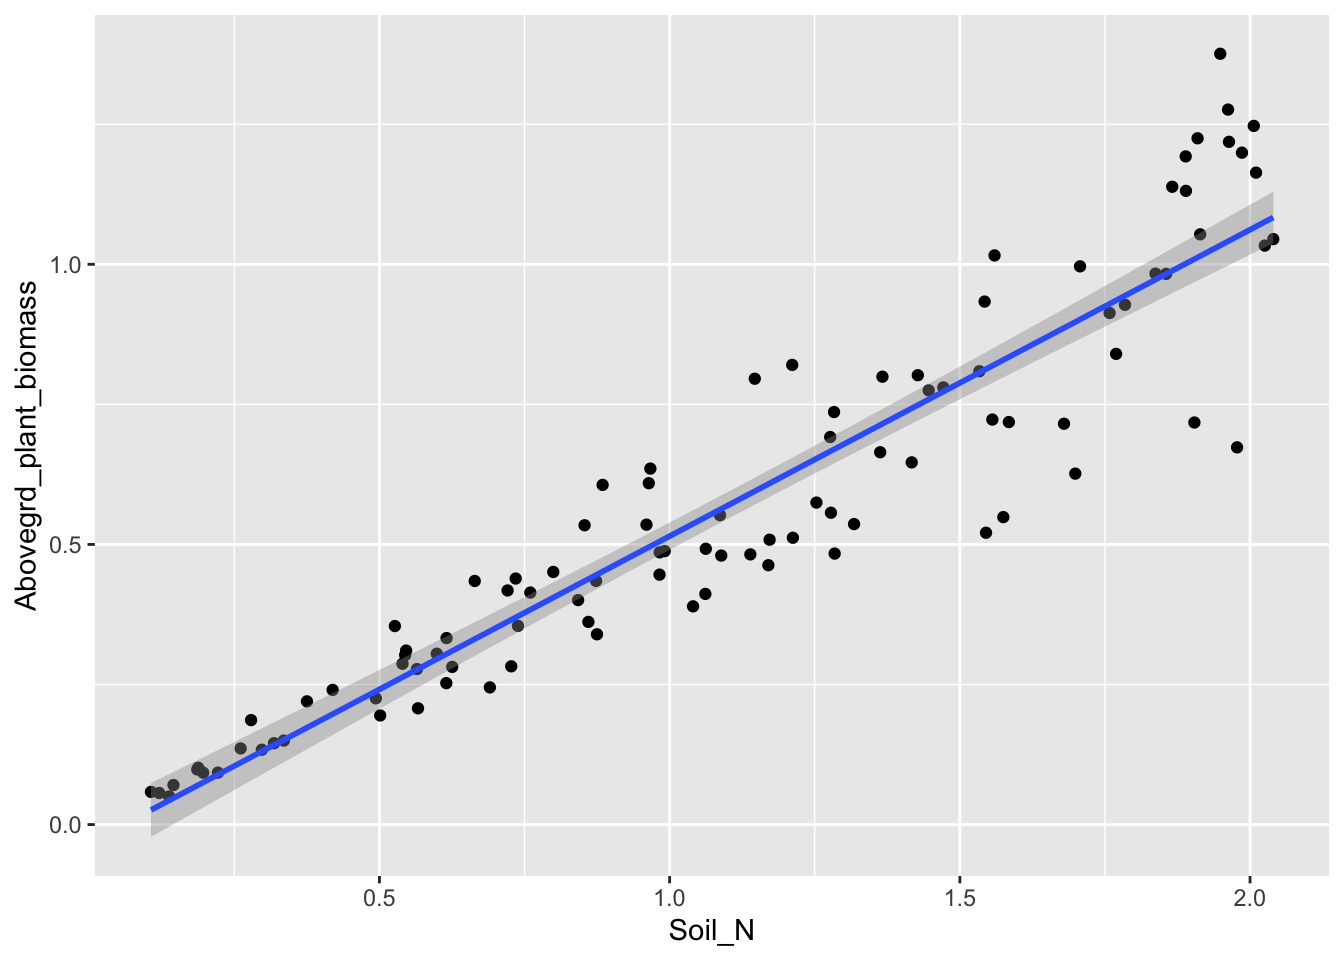
\includegraphics[width=0.9\linewidth]{/Users/stevenmh/MyDrive/Projects/ecosystems-primer/figs/anpp-1} \caption{*A statistical model of aboveground plant biomass as a function of available soil nitrogen.*}\label{fig:anpp}
\end{figure}

\begin{Shaded}
\begin{Highlighting}[]
\NormalTok{knitr}\OperatorTok{::}\KeywordTok{include_graphics}\NormalTok{(}\StringTok{"figs/LakeEcosystemCarpenteretal1992.png"}\NormalTok{)}
\end{Highlighting}
\end{Shaded}

\begin{figure}
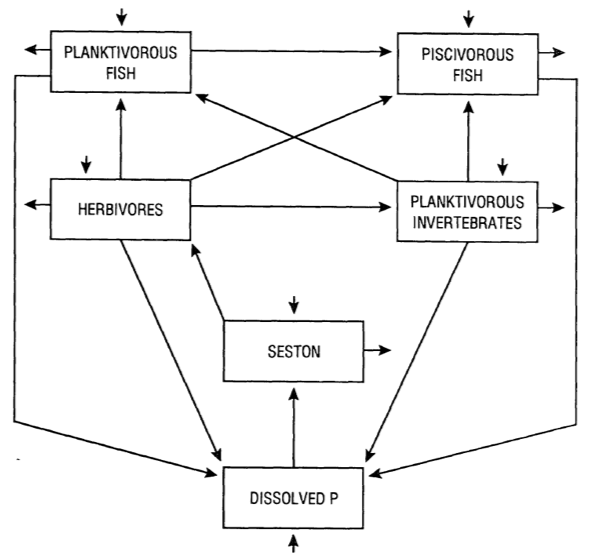
\includegraphics[width=1\linewidth]{figs/LakeEcosystemCarpenteretal1992} \caption{*Compartment models of other stuff*}\label{fig:compartment2}
\end{figure}

We model to aid understanding, because, at some level, the model is a quantitative and qualitative explanation for some phenomenon. We can use models to test hypotheses, guide experiments, and predict manage ecosystems and populations.

Statistical models (e.g., regression) are concerned with describing patterns and hypothesis testing. Process models (e.g., stock and flow models) are also descriptions of natural systems, but they include more mechanism and seek to describe mechanism and understand process. People sometimes call these \emph{mechanistic} models.

A theory is a well supported hierarchical framework that contains clearly formulated postulates, based on a minimal set of assumptions, from which a set of predictions logically follows \citep{Marquet2014}. \emph{Efficient} theory is based to as much as possible on first principles, and relies on as few assumptins as possible.

In contrast to theory, models are specific implementations of theory and specific descriptions of nature. Remember that in principle, \emph{all models are wrong, but some are useful}\footnote{Box, G. E. P. (1979), ``Robustness in the strategy of scientific model building'', in Launer, R. L.; Wilkinson, G. N., Robustness in Statistics, Academic Press, pp.~201--236.}.

\hypertarget{some-useful-terminology}{%
\section{Some useful terminology}\label{some-useful-terminology}}

\begin{itemize}
\tightlist
\item
  Domain and boundaries - the spatial, temporal and conceptual limits on a theory or model.
\item
  Spatial and temporal scale
\item
  State \emph{factors} are forcing functions, constraints, and outside influences
\item
  State \emph{variables} are pools or stocks, have one currency (e.g., kg, individuals), vary through time; stuff whose variation we model.
\item
  Flows = processes. They may be exchange between state variables (ecological, biogeochemical) such as ingestion, respiration, nutrient uptake; exchange with the external world we often refer to as transport, import, or export.
\item
  Parameters are typically fixed rate constants governing process/flows
\end{itemize}

\textbf{You might pause now}, and ask yourself ``is a lake a carbon sink or a source?'' Draw an appropriate compartment model to address this question. After having done so, ask yourself what assumptions you've made about the temporal and spatial scales. What mechanisms have you included? Why?

\hypertarget{model-making}{%
\section{Model making}\label{model-making}}

\hypertarget{describing-a-nitrogen-budget}{%
\chapter{Describing a nitrogen budget}\label{describing-a-nitrogen-budget}}

\begin{figure}
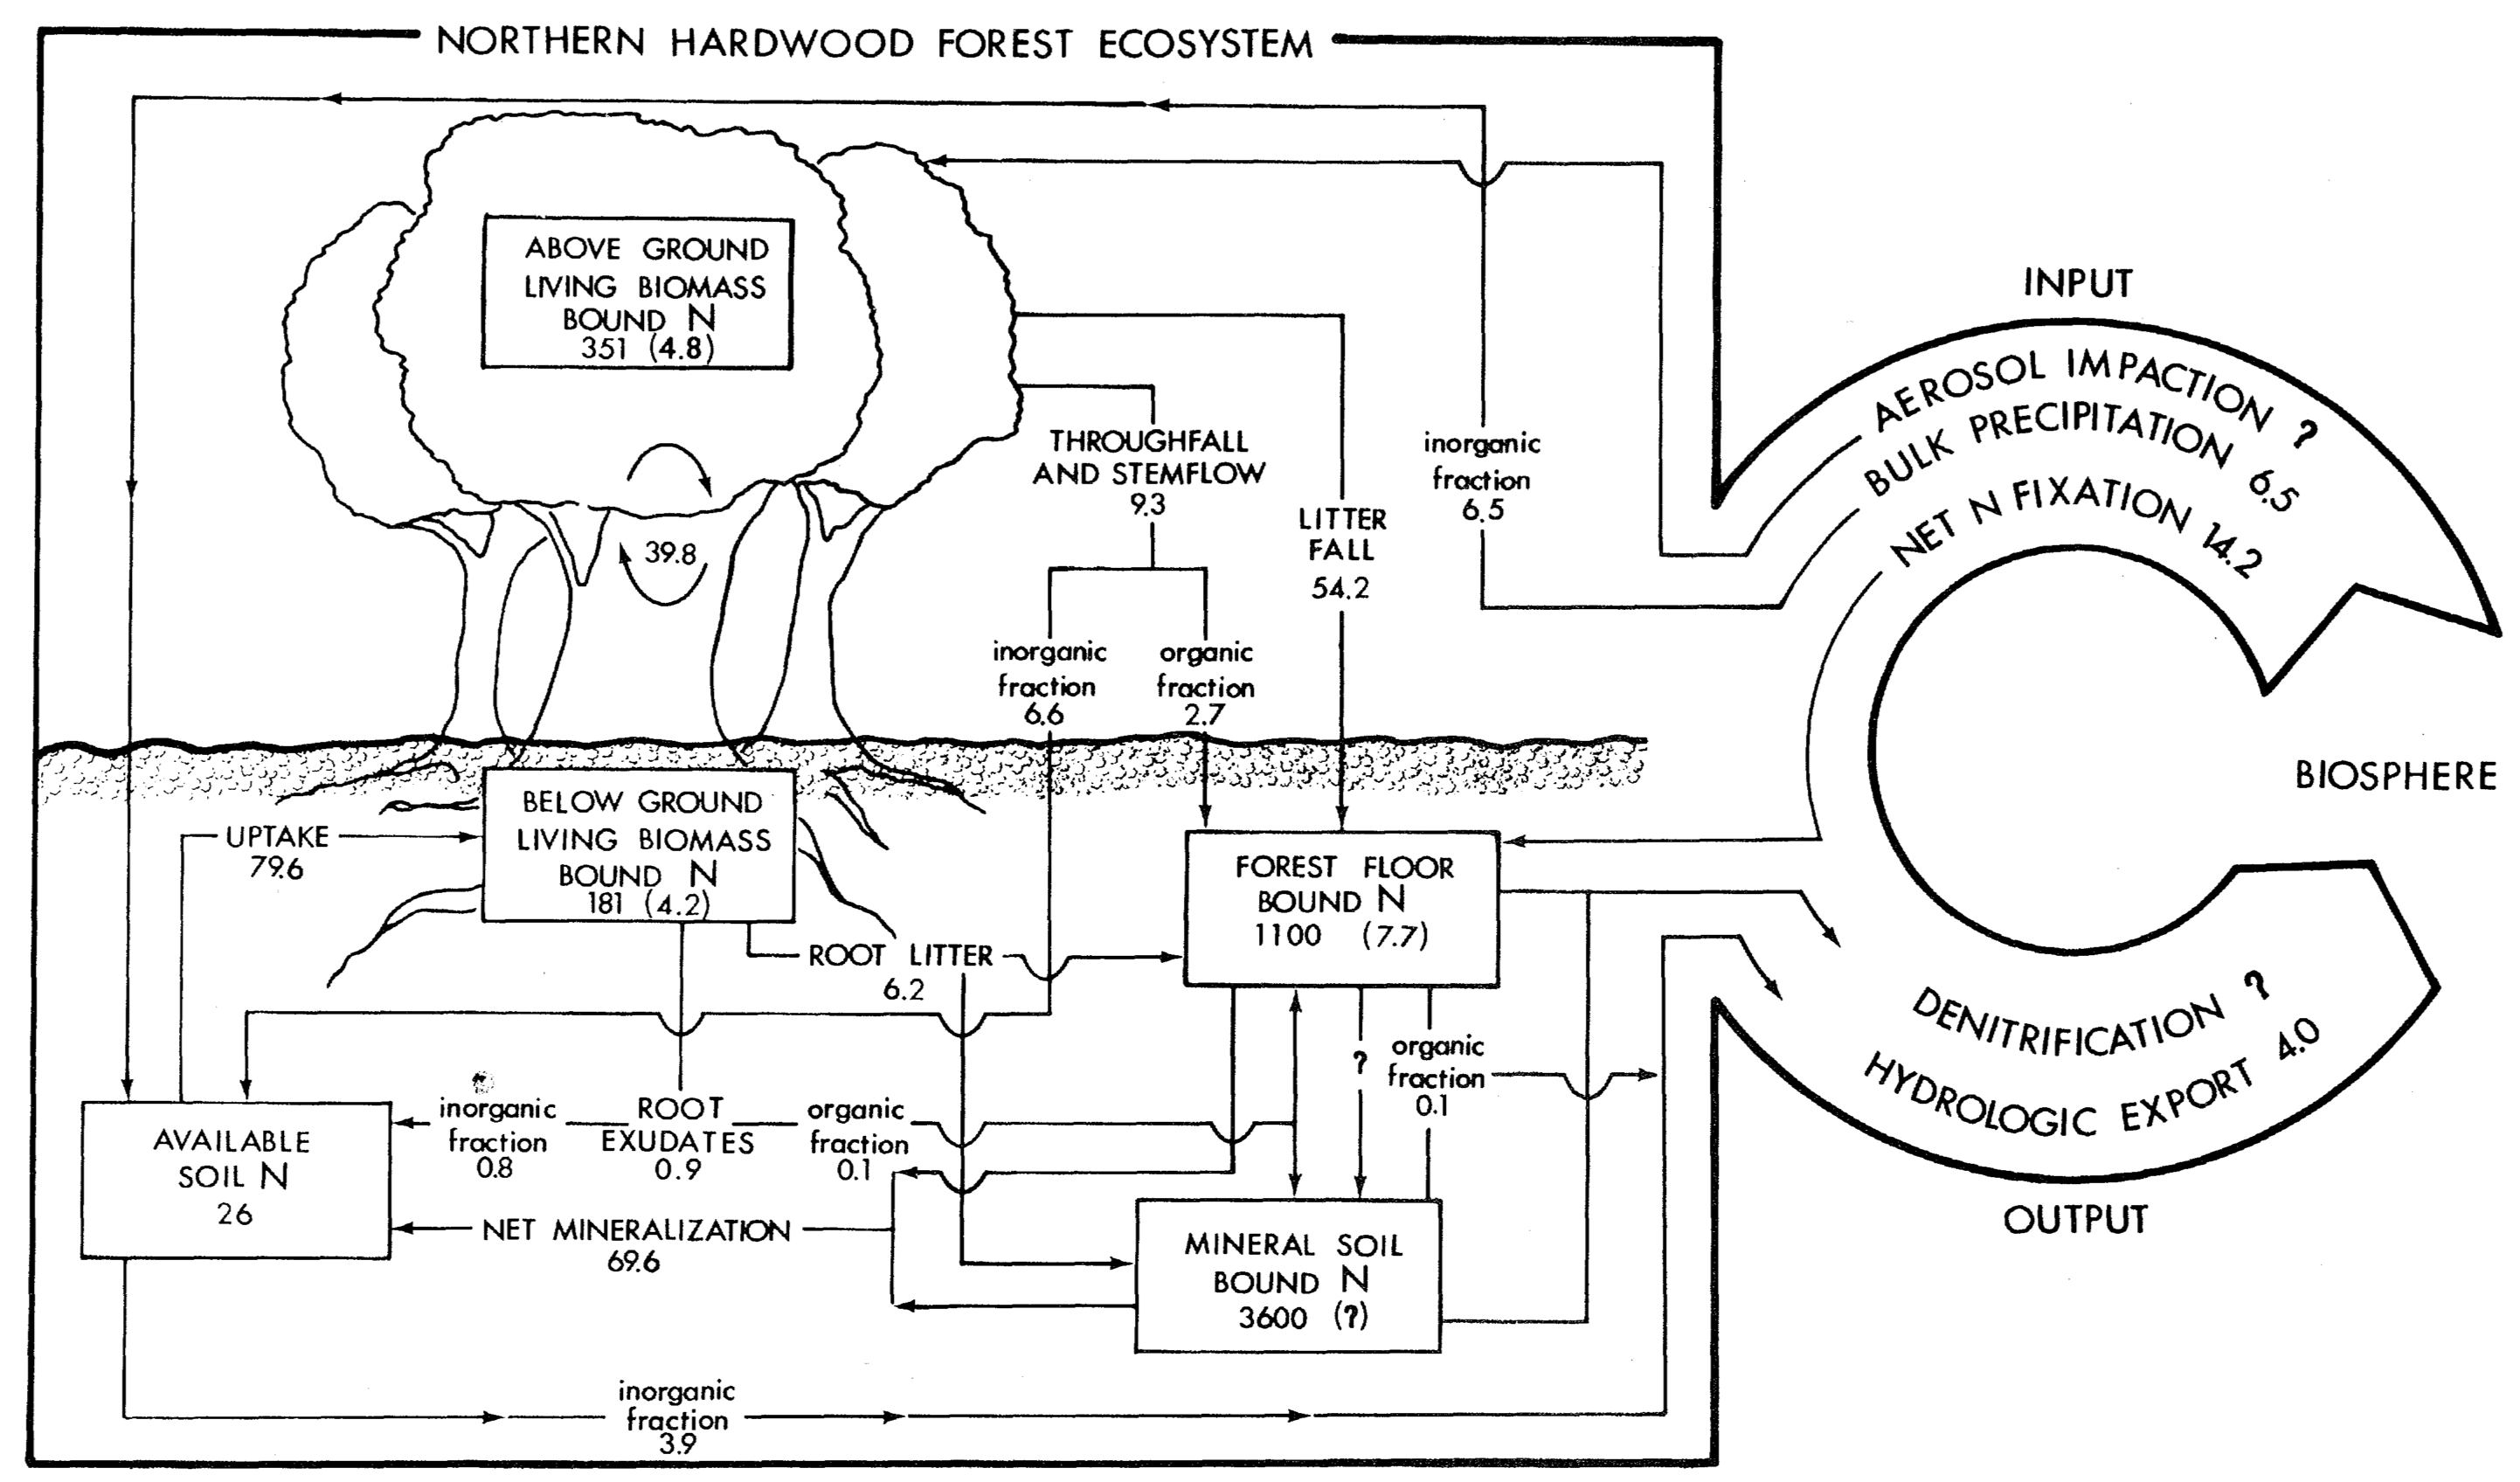
\includegraphics[width=1\linewidth]{figs/BormannF2} \caption{*Nitrogen bugdget for a temperate northern hardwood forest (Hubbard Brook Watershed 6, Bormann et al. 1977).*}\label{fig:hbnb}
\end{figure}

\begin{figure}
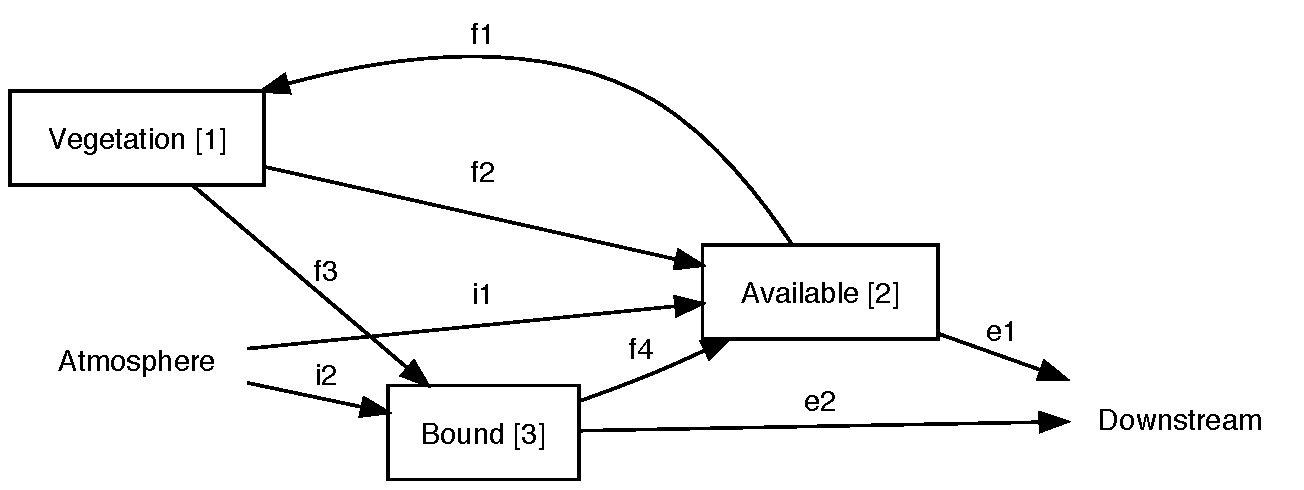
\includegraphics[width=0.9\linewidth]{figs/model3} \caption{*A simpler compartment model for Hubbard Brook Watershed 6, based on Bormann et al. (1977).*}\label{fig:hbnb3}
\end{figure}

\hypertarget{first-mathematical-form-for-plant-uptake}{%
\section{First mathematical form for plant uptake}\label{first-mathematical-form-for-plant-uptake}}

A common starting point for dynamics depending on two pools is the law of \emph{mass action}. This states that the reaction rate is proportional the product of the pools. In the case of plant uptake of N, which depends on the amounts of N in the available pool and the vegetation pool, this would be \(aVA\), where \(a\) is a proportionality constant. In some circumstances, these pools might also have exponents different than one, or \(aVA^2\). This occurs in chemistry when a reaction requires two molecules of ``A'' for each molecule of ``V''. It might occur in ecology if a rate depends differentially on A and B.

Use the law of mass action for plant uptake, we will describe the fluxes in the simple N budget above with the following expressions.

\begin{align}
\frac{dV}{dt} &= a_{1}AV - a_{2}V - a_3 V\\
\frac{dA}{dt} &= I_1 + a_{2}V +  a_{4}B - a_{5}A - a_{1}AV\\
\frac{dB}{dt} &= I_2 + a_{3}V - a_{4}B - a_{6}B
\end{align}

\hypertarget{paramaterization}{%
\section{Paramaterization}\label{paramaterization}}

Next, we find initial estimates for the parameters in our model. We use the
literature for this purpose.

If we have the data (we do) and relatively simple mathematical forms
(we do), it is fairly straightforward to estimate parameters. For
instance, we decided that net mineralization would be directly
proportional to the size of the organic pool, \(B\), that is, \(F_4 = a_4B\). To calculate \(a_4\), we substitute data where we can, and solve
what we need.
\begin{align*}
  F_2 &= a_4 B\\
  69.6 &= a_4 4700 \\
  a_4 &= \frac{69.6}{4700}\\
  a_4 &\approx 0.015
\end{align*}
We use the same approach for second order equations as well.

\begin{table*}
\caption{Parameters, variables, units and estimates for a simplified model of Bormann et al. (1977). All fluxes ($dX/dy$) are in units of kg\,ha$^{-1}$\,y$^{-1}$. (Note that calculations should not be included in your final table, but are presented here for comparison to your own calculations.) } 
\begin{tabular}{lcc} \hline \hline
$\mathbf{p}$, $\mathbf{V}$ & \textbf{unit} & \textbf{Estimate}\\ 
\hline
$A,\,B,\,V$ state variables & kg\,ha$^{-1}$ & 26, 4700, 532\\
$a_1$, uptake rate by V from A & (kg\,ha$^{-1}$)$^{-1}$\,y$^{-1}$  &  $79.6 / (26 \cdot 532) = 0.0058$\\
$a_2$, loss rate from V to A & y$^{-1}$ & $(6.6 + 0.8) / 532 = 0.014 $ \\
$a_3$, loss rate from V to B & (kg\,ha$^{-1}$)$^{-1}$\,y$^{-1}$ & $(54.2 + 2.7 + 0.1 + 6.2 ) / 532 = 0.00022 $ \\
$a_4$, mineralization & y$^{-1}$ & $ 69.6 / 4700 = 0.015$ \\
$a_5$, export from A & y$^{-1} $ & $ 3.9 /26 = 0.15$ \\
$a_6$, export from B & y$^{-1}$ & $0.1/4700 = 0.000021$ \\
$I_1$, bulk precip & kg\,ha$^{-1}$\,y$^{-1}$ & $ 6.5$ \\
$I_2$, N fixation & kg\,ha$^{-1}$\,y$^{-1}$ & $14.2$ 
\end{tabular}
\end{table*}

Enter parameters into R.

\begin{Shaded}
\begin{Highlighting}[]
\CommentTok{# Atmospheric inputs}
\CommentTok{##  Precip}
\NormalTok{i1 <-}\StringTok{ }\FloatTok{6.5}
\CommentTok{## fixation}
\NormalTok{i2 <-}\StringTok{ }\FloatTok{14.2}
\CommentTok{# uptake}
\NormalTok{a1 <-}\StringTok{ }\FloatTok{79.6} \OperatorTok{/}\StringTok{ }\NormalTok{(}\DecValTok{26} \OperatorTok{*}\StringTok{ }\DecValTok{532}\NormalTok{)}
\CommentTok{# throughfall and exudates (inorganic)}
\NormalTok{a2 <-}\StringTok{ }\NormalTok{(}\FloatTok{6.6} \OperatorTok{+}\StringTok{ }\FloatTok{0.8}\NormalTok{) }\OperatorTok{/}\StringTok{ }\DecValTok{532}
\CommentTok{# litter, throughfall, exudates (organic)}
\NormalTok{a3 <-}\StringTok{ }\NormalTok{(}\FloatTok{54.2} \OperatorTok{+}\StringTok{ }\FloatTok{2.7} \OperatorTok{+}\StringTok{ }\FloatTok{0.1} \OperatorTok{+}\StringTok{ }\FloatTok{6.2}\NormalTok{ ) }\OperatorTok{/}\StringTok{ }\DecValTok{532}
\CommentTok{# net mineralization}
\NormalTok{a4 <-}\StringTok{ }\FloatTok{69.6} \OperatorTok{/}\StringTok{ }\DecValTok{4700}
\CommentTok{# export from available}
\NormalTok{a5 <-}\StringTok{ }\FloatTok{3.9} \OperatorTok{/}\DecValTok{26}
\CommentTok{#export from bound}
\NormalTok{a6 <-}\StringTok{ }\FloatTok{0.1}\OperatorTok{/}\DecValTok{4700}

\CommentTok{# make a vector}
\NormalTok{params <-}\StringTok{ }\KeywordTok{c}\NormalTok{( }\DataTypeTok{a1 =}\NormalTok{ a1, }\DataTypeTok{a2 =}\NormalTok{ a2, }\DataTypeTok{a3 =}\NormalTok{ a3, }\DataTypeTok{a4 =}\NormalTok{ a4, }
            \DataTypeTok{a5 =}\NormalTok{ a5, }\DataTypeTok{a6 =}\NormalTok{ a6, }\DataTypeTok{i1 =}\NormalTok{ i1, }\DataTypeTok{i2 =}\NormalTok{ i2)}
\CommentTok{#...and look at it.}
\NormalTok{params}
\end{Highlighting}
\end{Shaded}

\begin{verbatim}
##           a1           a2           a3           a4           a5           a6 
## 5.754772e-03 1.390977e-02 1.187970e-01 1.480851e-02 1.500000e-01 2.127660e-05 
##           i1           i2 
## 6.500000e+00 1.420000e+01
\end{verbatim}

\hypertarget{mathematical-solution}{%
\section{Mathematical solution}\label{mathematical-solution}}

The \emph{mathematical solution} is the process of making the
predictions using our model and our parameters. We \emph{solve} the
model. With simple models, we can sometimes find analytical
solutions. For most ecosystem models, we have to solve the models
numerically using \emph{numerical integration}.

Here we write a function that includes our system of differential
equations. This will allow R to integrate change through time.

\begin{Shaded}
\begin{Highlighting}[]
\NormalTok{bormann1 <-}\StringTok{ }\ControlFlowTok{function}\NormalTok{(t, y, p) \{}
  \CommentTok{# time, vector of state variables and parameters must be in this order}
  \CommentTok{# we can use as.list for both the state variables and parameters}
  \CommentTok{# a1 = uptake}
  \CommentTok{# a2 = loss from veg to avail}
  \CommentTok{# a3 = loss from veg to bound}
  \CommentTok{# a4 = net mineralization}
  \CommentTok{# a5 = export from avail}
  \CommentTok{# a6 = export from bound}
  \KeywordTok{with}\NormalTok{( }\KeywordTok{as.list}\NormalTok{( }\KeywordTok{c}\NormalTok{(y, p) ), \{}
\NormalTok{    dV.dt <-}\StringTok{ }\NormalTok{a1 }\OperatorTok{*}\StringTok{ }\NormalTok{A }\OperatorTok{*}\StringTok{ }\NormalTok{V }\OperatorTok{-}\StringTok{ }\NormalTok{a2 }\OperatorTok{*}\StringTok{ }\NormalTok{V }\OperatorTok{-}\StringTok{ }\NormalTok{a3 }\OperatorTok{*}\StringTok{ }\NormalTok{V}
\NormalTok{    dA.dt <-}\StringTok{ }\NormalTok{i1 }\OperatorTok{+}\StringTok{ }\NormalTok{a2 }\OperatorTok{*}\StringTok{ }\NormalTok{V }\OperatorTok{+}\StringTok{ }\NormalTok{a4 }\OperatorTok{*}\StringTok{ }\NormalTok{B }\OperatorTok{-}\StringTok{ }\NormalTok{a1 }\OperatorTok{*}\StringTok{ }\NormalTok{A }\OperatorTok{*}\StringTok{ }\NormalTok{V }\OperatorTok{-}\StringTok{ }\NormalTok{a5 }\OperatorTok{*}\StringTok{ }\NormalTok{A }
\NormalTok{    dB.dt <-}\StringTok{ }\NormalTok{i2 }\OperatorTok{+}\StringTok{ }\NormalTok{a3 }\OperatorTok{*}\StringTok{ }\NormalTok{V }\OperatorTok{-}\StringTok{ }\NormalTok{a4 }\OperatorTok{*}\StringTok{ }\NormalTok{B }\OperatorTok{-}\StringTok{ }\NormalTok{a6 }\OperatorTok{*}\StringTok{ }\NormalTok{B }
    \CommentTok{# Here we return a list whose first element is the vector of}
    \CommentTok{# rates of change for the state variables. The first element must be these rates,}
    \CommentTok{# in the same order as the state variables in y}
    \CommentTok{# The second element is the total N in the system}
    \KeywordTok{return}\NormalTok{(}\KeywordTok{list}\NormalTok{( }\KeywordTok{c}\NormalTok{(dV.dt, dA.dt, dB.dt), }
                 \DataTypeTok{total =}\NormalTok{ V }\OperatorTok{+}\StringTok{ }\NormalTok{A }\OperatorTok{+}\StringTok{ }\NormalTok{B }
\NormalTok{                 )  )\})}
\NormalTok{\}}
\end{Highlighting}
\end{Shaded}

Now that we have the function, we tell R what to do with it. We will define the \emph{initial state of the system}, and then tell R which time point we want it to return.

The initial state of the system is the set of starting values for the state variables. We could choose any values, but I select the values given in Bormann et al.~(1977).

\begin{Shaded}
\begin{Highlighting}[]
\NormalTok{initial.state <-}\StringTok{ }\KeywordTok{c}\NormalTok{( }\DataTypeTok{V =} \DecValTok{532}\NormalTok{, }\DataTypeTok{A =} \DecValTok{26}\NormalTok{, }\DataTypeTok{B =} \DecValTok{4700}\NormalTok{)}
\end{Highlighting}
\end{Shaded}

\hypertarget{calibration-take-1}{%
\section{Calibration, take 1}\label{calibration-take-1}}

Calibration, in general, is the process of finding better estimates
for our parameters. We can do that by looking into the literature, or
by using independent data to estimates parameters directly.

If we take a look at the model output (above), we see both differences
and similarities with Bormann et al.~What are they?

What if we run it out longer, say, 100 years?

\begin{Shaded}
\begin{Highlighting}[]
\NormalTok{time <-}\StringTok{ }\DecValTok{0}\OperatorTok{:}\DecValTok{250}
\NormalTok{out <-}\StringTok{ }\KeywordTok{ode}\NormalTok{(}\DataTypeTok{y =}\NormalTok{ initial.state, }\DataTypeTok{times=}\NormalTok{time, }\DataTypeTok{func=}\NormalTok{bormann1, }\DataTypeTok{parms =}\NormalTok{ params)}
\KeywordTok{head}\NormalTok{(}\KeywordTok{round}\NormalTok{(out,}\DecValTok{1}\NormalTok{))}
\end{Highlighting}
\end{Shaded}

\begin{verbatim}
##      time     V    A      B  total
## [1,]    0 532.0 26.0 4700.0 5258.0
## [2,]    1 540.8 25.8 4708.2 5274.7
## [3,]    2 548.8 25.5 4717.2 5291.5
## [4,]    3 556.0 25.2 4727.0 5308.3
## [5,]    4 562.6 25.0 4737.5 5325.1
## [6,]    5 568.6 24.8 4748.6 5342.0
\end{verbatim}

\begin{Shaded}
\begin{Highlighting}[]
\CommentTok{#plot(out)}
\end{Highlighting}
\end{Shaded}

Use \texttt{gather()} and \texttt{ggplot()} to make a graph. We use \texttt{gather()} gather multiple columns into one with a new name (\texttt{value=kg.N}), keeping track of the names of the original columns in a new column (\texttt{key=State.var}). We can use \texttt{spread()} if we ever want to spread those columns back out.

\begin{Shaded}
\begin{Highlighting}[]
\NormalTok{outg <-}\StringTok{ }\KeywordTok{gather}\NormalTok{(}\KeywordTok{as.data.frame}\NormalTok{(out), }\DataTypeTok{key=}\NormalTok{State.var, }\DataTypeTok{value=}\NormalTok{kg.N, }
\NormalTok{              V, A, B, total, }\OperatorTok{-}\NormalTok{time,}
              \DataTypeTok{factor_key=}\OtherTok{TRUE}\NormalTok{)}
\KeywordTok{ggplot}\NormalTok{(outg, }\KeywordTok{aes}\NormalTok{(}\DataTypeTok{x=}\NormalTok{time, }\DataTypeTok{y=}\NormalTok{kg.N)) }\OperatorTok{+}\StringTok{ }\KeywordTok{geom_line}\NormalTok{() }\OperatorTok{+}\StringTok{ }\KeywordTok{facet_wrap}\NormalTok{(}\OperatorTok{~}\NormalTok{State.var, }\DataTypeTok{scale=}\StringTok{"free_y"}\NormalTok{)}
\end{Highlighting}
\end{Shaded}

\begin{figure}
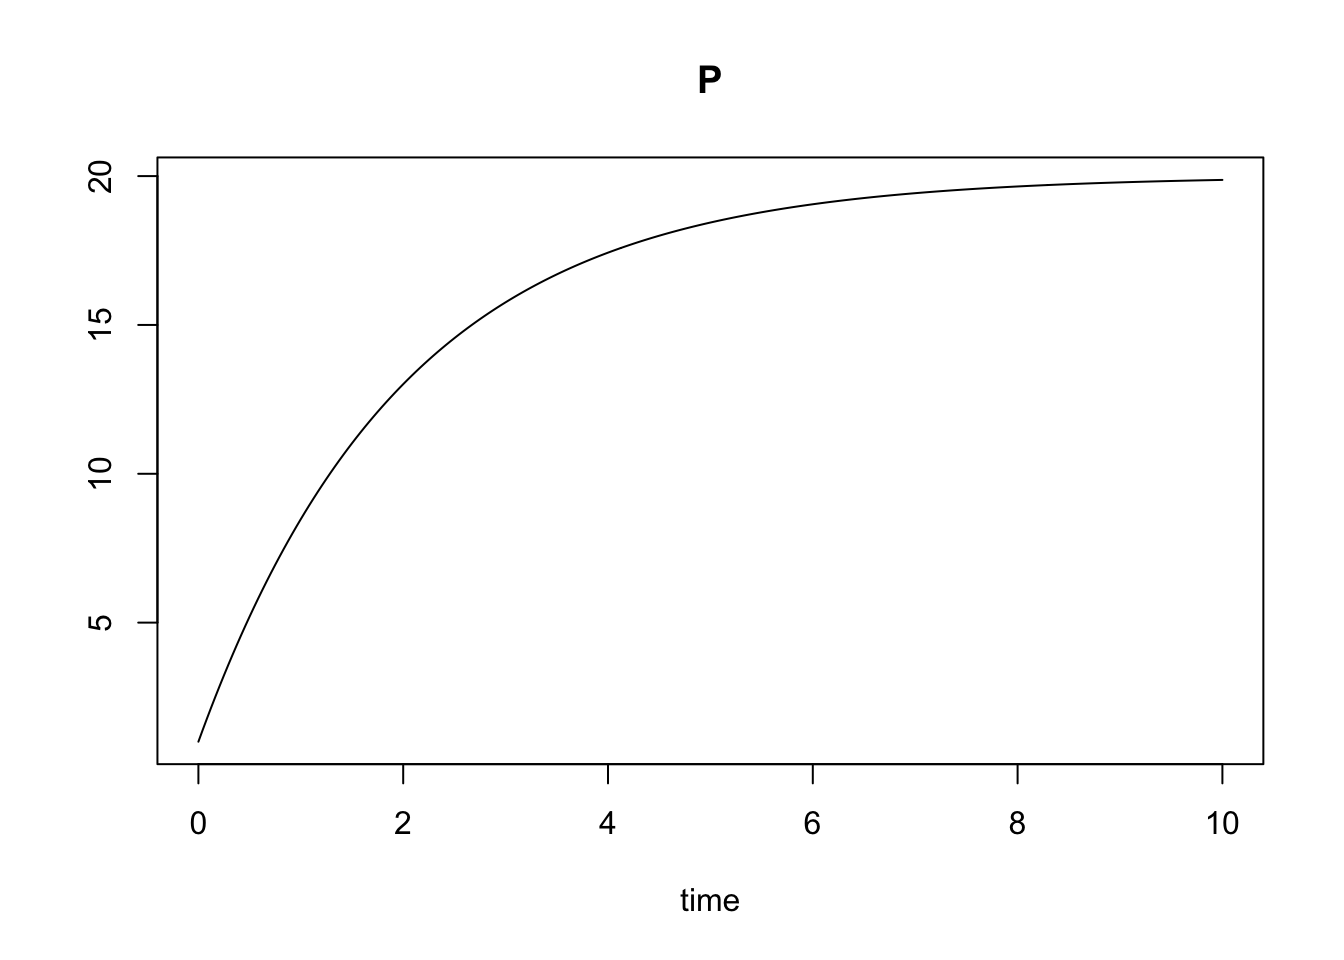
\includegraphics[width=0.9\linewidth]{/Users/stevenmh/MyDrive/Projects/ecosystems-primer/figs/unnamed-chunk-5-1} \caption{Dynamics of a simple N budget, based on Bormann et al. (1977).}\label{fig:unnamed-chunk-5}
\end{figure}

In some ways, we have been moderately successful in our first pass at
converting a purely budgetary model into a dynamic process model. We
mimicked total load, and see similar changes through time of all the
state variables.

\textbf{Questions to ponder}

We replicated approximately the N budget of Bormann et al.~(1977), but
clearly vegetation cannot keep accumulating N indefinitely.

What are our next steps? One logical step is to assume that as vegetation eventually gets limited by some factor or resource that is not in our model. If, at first approximation, the vegetation reaches a carrying capacity independent of high resource availability, we can use an approximation suggested by Soetaert and Hermann (2009) for \emph{self-limitation},
\[f(X)V\left(1-\frac{V}{K}\right)\]
where \(f(X)\) is everything else that regulates mass-specific growth rate.

\textbf{Exercise}

Include self-limitation in your model of vegetation, estimate \(K\), and produce output.

\hypertarget{budget-take-ii}{%
\section{Budget, take II}\label{budget-take-ii}}

Remember that following our template, we have a maximum rate times resource and self limitation, and inhibition. Currently, we have
\[\frac{dV}{dt} = a_{1}AV - a_{2}V - a_3 V\]
and rearranging,
\[\frac{dV}{dt} = \left(a_{1}A - a_{2} - a_3\right) V\]
If we add self-limitation, we get
\[\frac{dV}{dt} = \left(a_{1}A - a_{2} - a_3\right) V \left(1-\frac{V}{K}\right)\]
where \(K\) is the maximum amount of live vegetation that the ecosystem can sustain, in kg,N,ha\(^{-1}\). We don't know exactly what that is yet, but we may be able to get estimates from the literature. For know we can pretend that it is just a bit more than was there in the mid-1970s, say, \(K=600\).

Now we rewrite the R function with self-limitation.

\begin{Shaded}
\begin{Highlighting}[]
\NormalTok{bormann2 <-}\StringTok{ }\ControlFlowTok{function}\NormalTok{(t, y, p) \{}
  \CommentTok{# time, vector of state variables and parameters must be in this order}
  \CommentTok{# we can use as.list for both the state variables and parameters}
  \CommentTok{# a1 = uptake}
  \CommentTok{# a2 = loss from veg to avail}
  \CommentTok{# a3 = loss from veg to bound}
  \CommentTok{# a4 = net mineralization}
  \CommentTok{# a5 = export from avail}
  \CommentTok{# a6 = export from bound}
  \KeywordTok{with}\NormalTok{( }\KeywordTok{as.list}\NormalTok{( }\KeywordTok{c}\NormalTok{(y, p) ), \{}
\NormalTok{    dV.dt <-}\StringTok{ }\NormalTok{(a1 }\OperatorTok{*}\StringTok{ }\NormalTok{A  }\OperatorTok{-}\StringTok{ }\NormalTok{a2  }\OperatorTok{-}\StringTok{ }\NormalTok{a3) }\OperatorTok{*}\StringTok{ }\NormalTok{V }\OperatorTok{*}\StringTok{ }\NormalTok{(}\DecValTok{1}\OperatorTok{-}\NormalTok{V}\OperatorTok{/}\NormalTok{K)}
\NormalTok{    dA.dt <-}\StringTok{ }\NormalTok{i1 }\OperatorTok{+}\StringTok{ }\NormalTok{a2 }\OperatorTok{*}\StringTok{ }\NormalTok{V }\OperatorTok{+}\StringTok{ }\NormalTok{a4 }\OperatorTok{*}\StringTok{ }\NormalTok{B }\OperatorTok{-}\StringTok{ }\NormalTok{a1 }\OperatorTok{*}\StringTok{ }\NormalTok{A }\OperatorTok{*}\StringTok{ }\NormalTok{V }\OperatorTok{-}\StringTok{ }\NormalTok{a5 }\OperatorTok{*}\StringTok{ }\NormalTok{A }
\NormalTok{    dB.dt <-}\StringTok{ }\NormalTok{i2 }\OperatorTok{+}\StringTok{ }\NormalTok{a3 }\OperatorTok{*}\StringTok{ }\NormalTok{V }\OperatorTok{-}\StringTok{ }\NormalTok{a4 }\OperatorTok{*}\StringTok{ }\NormalTok{B }\OperatorTok{-}\StringTok{ }\NormalTok{a6 }\OperatorTok{*}\StringTok{ }\NormalTok{B }
    \CommentTok{# Here we return a list whose first element is the vector of}
    \CommentTok{# rates of change for the state variables. The first element must be these rates,}
    \CommentTok{# in the same order as the state variables in y}
    \CommentTok{# The second element is the total N in the system}
    \KeywordTok{return}\NormalTok{(}\KeywordTok{list}\NormalTok{( }\KeywordTok{c}\NormalTok{(dV.dt, dA.dt, dB.dt), }
                 \DataTypeTok{total =}\NormalTok{ V }\OperatorTok{+}\StringTok{ }\NormalTok{A }\OperatorTok{+}\StringTok{ }\NormalTok{B }
\NormalTok{                 )  )\})}
\NormalTok{\}}
\end{Highlighting}
\end{Shaded}

We can add a new parameter to our vector of parameters, and then solve our new function \texttt{bormann2} for the same time interval, and plot it.

\begin{Shaded}
\begin{Highlighting}[]
\NormalTok{params[}\StringTok{"K"}\NormalTok{] <-}\StringTok{ }\DecValTok{600}
\NormalTok{out <-}\StringTok{ }\KeywordTok{ode}\NormalTok{(}\DataTypeTok{y =}\NormalTok{ initial.state, }\DataTypeTok{times=}\NormalTok{time, }\DataTypeTok{func=}\NormalTok{bormann2, }\DataTypeTok{parms =}\NormalTok{ params)}
\NormalTok{outg <-}\StringTok{ }\KeywordTok{gather}\NormalTok{(}\KeywordTok{as.data.frame}\NormalTok{(out), }\DataTypeTok{key=}\NormalTok{State.var, }\DataTypeTok{value=}\NormalTok{kg.N, }
\NormalTok{              V, A, B, total, }\OperatorTok{-}\NormalTok{time,}
              \DataTypeTok{factor_key=}\OtherTok{TRUE}\NormalTok{)}
\KeywordTok{ggplot}\NormalTok{(outg, }\KeywordTok{aes}\NormalTok{(time, kg.N)) }\OperatorTok{+}\StringTok{ }\KeywordTok{geom_line}\NormalTok{() }\OperatorTok{+}\StringTok{ }\KeywordTok{facet_wrap}\NormalTok{(}\OperatorTok{~}\NormalTok{State.var, }\DataTypeTok{scale=}\StringTok{"free_y"}\NormalTok{)}
\end{Highlighting}
\end{Shaded}

\begin{figure}
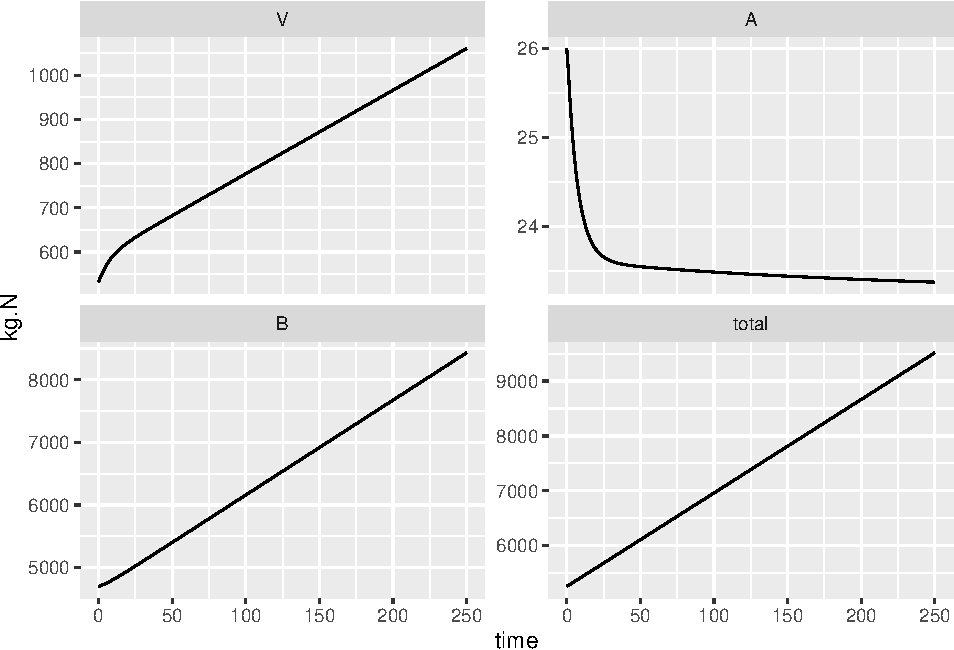
\includegraphics[width=0.9\linewidth]{/Users/stevenmh/MyDrive/Projects/ecosystems-primer/figs/unnamed-chunk-6-1} \caption{Dynamics of an N budget, assuming density-dependence in vegetation with a fixed carrying capacity (Bormann et al. 1977).}\label{fig:unnamed-chunk-6}
\end{figure}

Unlike our first model of this system, we see state variables on curved trajectories and perhaps reaching asymptotes. This makes greater intuitive sense - over the short term, it is the same as the simple N budget shown in \citet{Bormann1977} and it also shows a reasonable longterm trajectory for the vegetation, and the predicted consequences for the available and bound pools.

\hypertarget{references}{%
\chapter{References}\label{references}}

  \bibliography{book.bib,packages.bib}

\end{document}
